%% For double-blind review submission
\documentclass[acmlarge,anonymous]{acmart}\settopmatter{printfolios=true}
%% For single-blind review submission
%\documentclass[acmlarge,review]{acmart}\settopmatter{printfolios=true}
%% For final camera-ready submission
%\documentclass[acmlarge]{acmart}\settopmatter{}

%% Some recommended packages.
\usepackage{booktabs}   %% For formal tables:
                        %% http://ctan.org/pkg/booktabs
\usepackage{subcaption} %% For complex figures with subfigures/subcaptions
                        %% http://ctan.org/pkg/subcaption

% Haskell code snippets and useful shortcuts
\usepackage{minted}
\setminted[haskell]{escapeinside=@@}
\newcommand{\hs}{\mintinline{haskell}}
\newcommand{\teq}{\smaller $\sim$}
\newcommand{\ghci}{$\lambda$>}
\newcommand{\defeq}{\stackrel{\text{def}}{=}}
\newcommand{\std}[1]{{\color[rgb]{0,0.3,0} #1}}
\newcommand{\blk}[1]{{\color[rgb]{0,0,0} #1}}

\makeatletter\if@ACM@journal\makeatother
%% Journal information (used by PACMPL format)
%% Supplied to authors by publisher for camera-ready submission
\acmJournal{PACMPL}
\acmVolume{1}
\acmNumber{1}
\acmArticle{1}
\acmYear{2017}
\acmMonth{1}
\acmDOI{10.1145/nnnnnnn.nnnnnnn}
\startPage{1}
\else\makeatother
%% Conference information (used by SIGPLAN proceedings format)
%% Supplied to authors by publisher for camera-ready submission
\acmConference[PL'17]{ACM SIGPLAN Conference on Programming Languages}{January 01--03, 2017}{New York, NY, USA}
\acmYear{2017}
\acmISBN{978-x-xxxx-xxxx-x/YY/MM}
\acmDOI{10.1145/nnnnnnn.nnnnnnn}
\startPage{1}
\fi


%% Copyright information
%% Supplied to authors (based on authors' rights management selection;
%% see authors.acm.org) by publisher for camera-ready submission
\setcopyright{none}             %% For review submission
%\setcopyright{acmcopyright}
%\setcopyright{acmlicensed}
%\setcopyright{rightsretained}
%\copyrightyear{2017}           %% If different from \acmYear

\bibliographystyle{ACM-Reference-Format}
\citestyle{acmauthoryear}   %% For author/year citations

\begin{document}

\title{Algebraic Graphs with Class}
                                        %% [Short Title] is optional;
                                        %% when present, will be used in
                                        %% header instead of Full Title.
%\titlenote{with title note}
                                        %% \titlenote is optional;
                                        %% can be repeated if necessary;
                                        %% contents suppressed with 'anonymous'
\subtitle{Functional Pearl}
                                        %% \subtitle is optional
%\subtitlenote{with subtitle note}      %% \subtitlenote is optional;
                                        %% can be repeated if necessary;
                                        %% contents suppressed with 'anonymous'

%% Author information
%% Contents and number of authors suppressed with 'anonymous'.
%% Each author should be introduced by \author, followed by
%% \authornote (optional), \orcid (optional), \affiliation, and
%% \email.
%% An author may have multiple affiliations and/or emails; repeat the
%% appropriate command.
%% Many elements are not rendered, but should be provided for metadata
%% extraction tools.

%% Author with single affiliation.
\author{First1 Last1}
\authornote{with author1 note}          %% \authornote is optional;
                                        %% can be repeated if necessary
\orcid{nnnn-nnnn-nnnn-nnnn}             %% \orcid is optional
\affiliation{
  \position{Position1}
  \department{Department1}              %% \department is recommended
  \institution{Institution1}            %% \institution is required
  \streetaddress{Street1 Address1}
  \city{City1}
  \state{State1}
  \postcode{Post-Code1}
  \country{Country1}
}
\email{first1.last1@inst1.edu}          %% \email is recommended

%% Paper note
%% The \thanks command may be used to create a "paper note" ---
%% similar to a title note or an author note, but not explicitly
%% associated with a particular element.  It will appear immediately
%% above the permission/copyright statement.
%\thanks{with paper note}               %% \thanks is optional
                                        %% can be repeated if necesary
                                        %% contents suppressed with 'anonymous'


%% Abstract
%% Note: \begin{abstract}...\end{abstract} environment must come
%% before \maketitle command
\begin{abstract}
The paper presents a minimalistic, elegant and powerful approach to working
with graphs in a functional programming language. We build on a rigorous
mathematical foundation --- an algebra of graphs --- that allows to apply
equational reasoning for proving the correctness of graph transformation
algorithms. Algebraic graphs allow to avoid partial functions, typically
required for handling `malformed graphs' that contain an edge referring to
a non-existent vertex. Such malformed graphs are impossible to specify
algebraically, which helps to liberate APIs of existing graph libraries
from partial functions.

We show that the algebra of graphs can represent directed, undirected, reflexive
and transitive graphs, as well as hypergraphs, by appropriately choosing
the set of underlying axioms. The flexibility of the approach is
demonstrated by a few examples, and by developing a library for construction
and transformation of polymorphic graphs.
\end{abstract}

%% 2012 ACM Computing Classification System (CSS) concepts
%% Generate at 'http://dl.acm.org/ccs/ccs.cfm'.
\begin{CCSXML}
<ccs2012>
<concept>
<concept_id>10002950.10003624.10003633</concept_id>
<concept_desc>Mathematics of computing~Graph theory</concept_desc>
<concept_significance>500</concept_significance>
</concept>
<concept>
<concept_id>10003752.10010124.10010125.10010127</concept_id>
<concept_desc>Theory of computation~Functional constructs</concept_desc>
<concept_significance>500</concept_significance>
</concept>
</ccs2012>
\end{CCSXML}

\ccsdesc[500]{Mathematics of computing~Graph theory}
\ccsdesc[500]{Theory of computation~Functional constructs}%% End of generated code

\keywords{algebra, graph theory, polymorphism, functional programming}

%% Note: \maketitle command must come after title commands, author
%% commands, abstract environment, Computing Classification System
%% environment and commands, and keywords command.
\maketitle

%!TEX root = alga.tex
\section{Introduction}\label{sec-intro}

Graphs are ubiquitous in computing, yet working with graphs often requires
painfully low-level fiddling with sets of vertices and edges. Building
high-level abstractions is difficult, because the commonly used
foundation -- the pair $(V, E)$ of vertex set $V$ and edge set $E$ -- is a source
of partial functions. If $E \nsubseteq V \times V$, the pair is inconsistent and
does not correspond to a graph. This inherent partiality often leaks through
abstractions in state-of-the-art Haskell\footnote{In this paper
we exclusively use Haskell, but the presented approach can be adapted to other
programming languages.} graph libraries.

For example, the \textsf{containers} library represents graphs by
\emph{adjacency arrays}~\cite{1995_king_graphs}. To construct a graph
one specifies the pair $(V,E)$, e.g.
\hs{buildG (1,3) [(1,2),(2,3)]} constructs the graph with $V=\{1,2,3\}$ and
$E=\{(1,2), (2,3)\}$. Note that \hs{buildG} is partial:
\hs{buildG (1,2) [(3,1)]} is well-typed but fails with the
\textsf{`index out of range'} error. Another popular library \textsf{fgl}
uses the \emph{inductive graph representation} by~\citet{2001_erwig_inductive},
but its graph construction API is also based on sets of vertices and edges and
has partial functions, e.g. \hs{insEdge} can fail with
the \textsf{`edge from non-existent vertex'} error. Both \textsf{containers}
and \textsf{fgl} are treasure troves of graph algorithms, but it is easy to make an
error when using them. One can wrap these libraries in a safe interface, but the
question is: What is the right interface for constructing graphs? Is there a better
foundation than the pair $(V, E)$?

We present \emph{algebraic graphs} --- a new interface
for graph construction and transformation. We abstract away from graph representation
details and characterise graphs and two operations on them by a set of axioms,
much like numbers with addition and multiplication are algebraically characterised
by \emph{rings}~\cite{1999_maclane_algebra}. The presented approach is inspired by the
\emph{algebra of parameterised graphs}, a mathematical formalism used in digital
circuit design~\cite{2014_algebra_mokhov}, which we distil and adapt to the context
of functional programming.

The two binary operations on algebraic graphs, called \emph{overlay} and \emph{connect},
have two important properties: i) they are closed on the set of graphs, i.e. are total
functions, and ii) they can be used to construct any graph starting from the \emph{empty} and
single-\emph{vertex} graphs. This leads us to the safe and minimalistic core of four graph
construction primitives, as captured by the following data type:

\begin{minted}{haskell}
data Graph a = Empty
             | Vertex a
             | Overlay (Graph a) (Graph a)
             | Connect (Graph a) (Graph a)
\end{minted}

\noindent
To make the core more reusable we also define the following type class\footnote{The
name collision is not a problem in practice, because the data type and type class
are not used together and can be defined in separate modules.}, whose
instances must obey the axioms of the algebra:

\begin{minted}{haskell}
class Graph g where
    type Vertex g
    empty   :: g
    vertex  :: Vertex g -> g
    overlay :: g -> g -> g
    connect :: g -> g -> g
\end{minted}

\noindent
The main idea of the paper is that this simple core is as a solid foundation for
working with graphs. The type class has classic inhabitants, such as the pair $(V,E)$,
data types from \textsf{containers} and \textsf{fgl}, as well as new, unknown forms
of life. Our contributions are:
\begin{itemize}
  \item Compared to existing libraries, algebraic graphs have a smaller
  core (just four graph construction primitives), are more compositional
  (hence greater code reuse), and have no partial functions (hence fewer
  opportunities for usage errors). We present the core and justify these claims
  in \S\ref{sec-core}.

  \item The core has a simple mathematical structure fully characterised
  by a set of axioms~(\S\ref{sec-algebra}). This makes the
  proposed interface easier for testing and formal verification. We show that
  the core is \emph{complete}, i.e. any graph can be constructed, and \emph{sound},
  i.e. malformed graphs cannot be constructed.

  \item Under the basic set of axioms, algebraic graphs correspond to directed
  graphs with no edge labels. As we show in~\S\ref{sec-a-la-carte}, by extending
  the algebra
  with additional axioms, it is possible to also represent undirected, reflexive
  and transitive graphs, their combinations, as well as hypergraphs.
%   Importantly, the core
%   graph construction primitives remain unchanged, which allows to define highly
%   reusable polymorphic functions on graphs.

  \item We develop a library\footnote{The library is on Hackage:
  \url{http://hackage.haskell.org/package/algebraic-graphs}.} for polymorphic graph
  construction and transformation on top of the algebraic core and
  demonstrate its flexibility in \S\ref{sec-transformations}.
  % Although the development of efficient algorithms for algebraic
  % graphs is outside the scope of this paper, we show that the library can cope
  % with graphs comprising billions of edges in the matter of
  % seconds, which is sufficiently fast for many applications.
\end{itemize}

Graphs and functional programming have a long history. We review related
work in \S\ref{sec-related}. Limitations of this work and future
research directions are discussed in \S\ref{sec-discussion}.

%!TEX root = alga.tex
\vspace{-0.5mm}
\section{The Core}\label{sec-core}
In this section we define the \emph{core} of algebraic graphs comprising
four graph construction primitives. We describe the semantics of the primitives
using the common representation of graphs by sets of vertices and edges, and
then abstract away from this representation by focusing on the laws that these
primitives satisfy.

Let $G$ be the set of all directed graphs whose vertices come from a fixed
universe $\mathbb{V}$. As an example, we can think of graphs whose vertices are
positive integers. A graph $g \in G$ can be represented by a pair $(V, E)$ where
$V\subseteq \mathbb{V}$ is the set of its vertices and $E \subseteq V \times V$ is
the set of its edges. As mentioned in~\S\ref{sec-intro}, when $E \nsubseteq V \times V$
the pair $(V, E)$ is inconsistent and does not correspond to a graph.

When one needs to guarantee the internal consistency of a data structure, the standard
solution is to define an abstract interface that encapsulates the data structure and
provides a set of safe construction primitives. This is exactly the approach we take.

\subsection{Constructing Graphs}\label{sub-constructing}

The simplest possible graph is the \emph{empty} graph. We denote it by
$\varepsilon$, therefore $\varepsilon = (\varnothing, \varnothing)$ and
$\varepsilon \in G$. A graph with a \emph{single vertex} $v \in \mathbb{V}$
is denoted simply by $v$. For example, $1 \in G$ is the graph
$({1}, \varnothing)$.

To construct larger graphs from the above primitives we define binary
operations \emph{overlay} and \emph{connect}, denoted by $+$ and $\rightarrow$,
respectively. The overlay operation $+$ is defined as
\[
(V_1, E_1) + (V_2, E_2)~~\defeq~~(V_1 \cup V_2, E_1 \cup E_2).
\]
That is, the overlay of two graphs comprises the union of their vertices and edges.
The connect $\rightarrow$ operation is defined similarly:
\[
(V_1, E_1) \rightarrow (V_2, E_2)~~\defeq~~(V_1 \cup V_2, E_1 \cup E_2 \cup V_1 \times V_2).
\]
The difference is that when we connect two graphs, an edge is added from each
vertex of the left-hand argument to each vertex of the right-hand
argument\footnote{Our definitions of overlay and connect coincide
with those of graph \emph{union} and \emph{join}, respectively,
e.g see~\citet{1969_graph_theory_harary},
however the arguments of union and join are typically assumed to have disjoint
sets of vertices. We make no such assumptions, hence our definitions are total:
any graphs can be composed using overlay and connect.}.
Note that the connect operation is the only source of edges when constructing
graphs. As we will see in~\S\ref{sec-algebra}, overlay and connect
are very similar to addition and multiplication. We therefore give connect a higher
precedence, i.e. $1 + 2 \rightarrow 3$ is interpreted as $1 + (2 \rightarrow 3)$.
Fig.~\ref{fig-construction} illustrates a few examples of graph construction
using the defined primitives:
\begin{itemize}
  \item $1 + 2$ is the graph with two isolated vertices 1 and 2.
  \item $1 \rightarrow 2$ is the graph with an edge between vertices 1 and 2.
  \item $1 \rightarrow (2 + 3)$ comprises vertices $\{1, 2, 3\}$
  and edges $\{(1, 2), (1, 3)\}$.
  \item $1 \rightarrow 1$ is the graph with vertex 1 and the \emph{self-loop}.
  \item $1 \rightarrow 2 + 2 \rightarrow 3$ is the \emph{path graph} on vertices $\{1, 2, 3\}$.
\end{itemize}

As shown in~\S\ref{sec-intro}, the core can be represented by a simple
data type \hs{Graph}, parameterised by the type of vertices~\hs{a}.
To make the core more reusable, the next subsection defines the core type class that
has the usual inhabitants, such as the pair $(V,E)$, data types from
\textsf{containers} and \textsf{fgl}, as well as other, stranger forms of life.

\subsection{Type Class}\label{sub-class}

We abstract the graph construction primitives defined in \S\ref{sub-constructing}
as the type class \hs{Graph}\footnote{The name collision (\hs{data Graph}
and \hs{class Graph}) is not a problem in practice, because the data type and type class
are not used together and live in separate modules.}:

\begin{minted}{haskell}
class Graph g where
    type Vertex g
    empty   :: g
    vertex  :: Vertex g -> g
    overlay :: g -> g -> g
    connect :: g -> g -> g
\end{minted}

\noindent
Here the associated type\footnote{Associated
types~\cite{2005_associated_type_chakravarty} require the \textsf{TypeFamilies}
GHC extension.} \hs{Vertex@\,\blk{g}@} corresponds to the universe of graph
vertices $\mathbb{V}$, \hs{empty} is the empty graph
$\varepsilon$, \hs{vertex} constructs a graph with a single vertex,
and \hs{overlay} and \hs{connect} compose given graphs according to
the definitions in~\S\ref{sub-constructing}. All methods of the type class
are total, i.e. are defined for all possible inputs, therefore,
the presented API allows \emph{fewer opportunities for usage errors}
and \emph{greater opportunities for reuse}.

Let us put the interface to the test and construct some graphs. A single edge is
obtained by connecting two vertices:

\begin{minted}{haskell}
edge :: Graph g => Vertex g -> Vertex g -> g
edge x y = connect (vertex x) (vertex y)
\end{minted}

\noindent
The graphs in Fig.~\ref{fig-construction}(b,d) are \hs{edge@\,@1@\,@2} and
\hs{edge@\,@1@\,@1}, respectively.
A graph that contains a given list of isolated vertices can be constructed
as follows:

\begin{minted}{haskell}
vertices :: Graph g => [Vertex g] -> g
vertices = @\std{foldr}@ overlay empty . @\std{map}@ vertex
\end{minted}

\noindent
That is, we turn each vertex into a singleton graph and overlay the results.
The graph in Fig.~\ref{fig-construction}(a) is \hs{vertices@\,@[1,2]}.
By replacing \hs{overlay} with \hs{connect} in the above
definition, we obtain a directed \emph{clique} -- a fully connected graph
on a given list of vertices:

\begin{minted}{haskell}
clique :: Graph g => [Vertex g] -> g
clique = @\std{foldr}@ connect empty . @\std{map}@ vertex
\end{minted}

\noindent
For example, \hs{clique@\,@[1,2,3]} expands to
$1 \rightarrow 2 \rightarrow 3 \rightarrow \varepsilon$, i.e.
the graph with three vertices $\{1, 2, 3\}$ and three edges $(1, 2)$, $(1, 3)$ and
$(2, 3)$. Note that it is different from the graph in Fig.~\ref{fig-construction}(e).

The graph construction functions defined above are total, fully polymorphic, and elegant.
Thanks to the minimalistic core type class, it is easy to wrap your favourite
graph library into the described interface, and reuse the above functions, as
well as many others that we define throughout this paper.

%!TEX root = alga.tex
\begin{figure*}
\begin{subfigure}[b]{0.4\linewidth}
\centerline{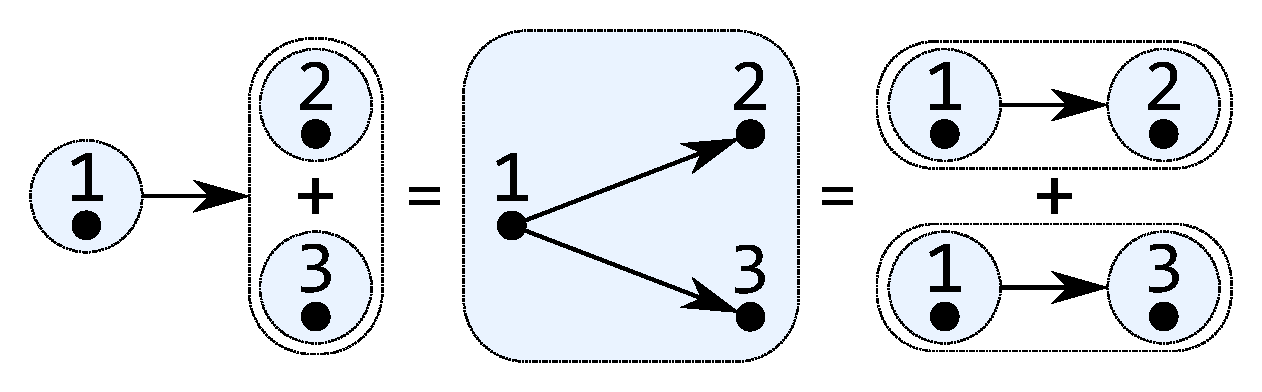
\includegraphics[scale=0.27]{fig/ax-distributivity.pdf}}
\caption{Distributivity: $1 \rightarrow (2 + 3) = 1 \rightarrow 2 + 1 \rightarrow 3$ }
\end{subfigure}
\hspace{12mm}
\begin{subfigure}[b]{0.5\linewidth}
\centerline{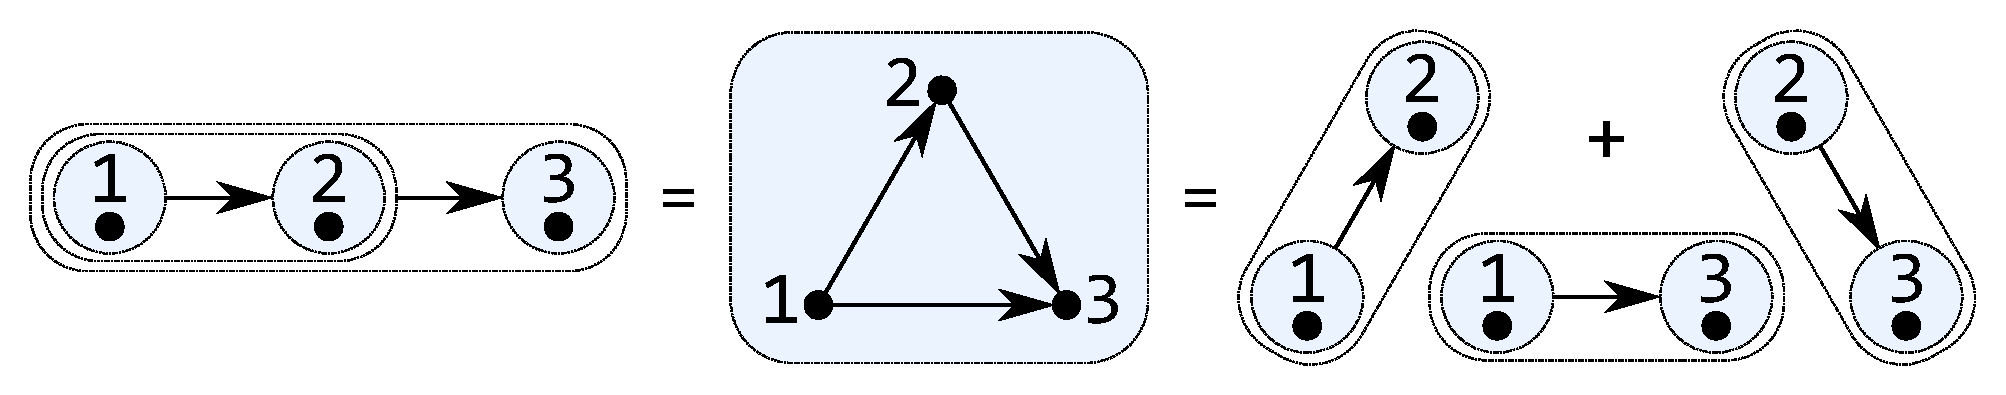
\includegraphics[scale=0.27]{fig/ax-decomposition.pdf}}
\caption{Decomposition: $1 \rightarrow 2 \rightarrow 3 = 1 \rightarrow 2 +
1 \rightarrow 3 + 2 \rightarrow 3$}
\end{subfigure}
\caption{Two axioms of the algebra of graphs\label{fig-axioms}}
\end{figure*}

\section{Algebraic structure}\label{sec-algebra}

The functions \hs{edge}, \hs{vertices} and \hs{clique} defined in the previous
section \S\ref{sec-core} satisfy a few properties that we can intuitively write down
and verify at the level of sets of vertices and edges:
\begin{itemize}
    \item \hs{vertex@\,\blk{x}@} $\ =\ $ \hs{vertices@\,@[x]} and
    \hs{edge@\,\blk{x}\,\blk{y}@} $\ =\ $ \hs{clique@\,@[x,y]}.
    \item \hs{vertices xs} $\ \subseteq\ $ \hs{clique xs}, where $x \subseteq y$ means
    $x$ is a \emph{subgraph} of $y$, i.e. $V_x\subseteq V_y$ and $E_x\subseteq E_y$ hold.
    \item \hs{clique@\,@(xs@\,@++@\,\blk{ys}@)} $\ =\ $ \hs{connect@\,@(}\hs{clique@\,\blk{xs}@)@\,@(}\hs{clique@\,\blk{ys}@)}.
\end{itemize}

In this section we characterise the \hs{Graph} type class with a set of
axioms that reveal an algebraic structure very similar to a semiring\footnote{
See~\citet{1999_semirings_golan} for a classic overview of semiring
applications, where the author hints at the existence of a non-semiring `algebra of
digraphs' whose operations coincide with overlay and connect, referring to an unpublished
paper by Anthony P. Stone. \citet{2013_semirings_dolan} uses the semiring theory to
implement graph algorithms.}.
This provides a convenient framework for proving graph properties, such as
those listed above, using equational reasoning. The presented characterisation is
generally useful for formal verification, as well as automated testing of graph library
APIs.

\subsection{Axiomatic characterisation}\label{sub-laws}

The definitions of \hs{vertices} and \hs{clique} in \S\ref{sub-class}
use $\varepsilon$ as the identity for both overlay $+$ and connect $\rightarrow$
operations. This seems unusual, but we can check that
$x + \varepsilon = x$ and $x \rightarrow \varepsilon = x$ for any graph $x \in G$
by plugging the empty graph into the definitions of overlay and connect,
respectively. Furthermore, we can verify the following:
\begin{itemize}
    \item $(G,+,\varepsilon)$ is an idempotent commutative monoid.
    \item $(G,\rightarrow,\varepsilon)$ is a monoid.
    \item $\rightarrow$ distributes over $+$, as illustrated
    in Fig.~\ref{fig-axioms}(a).
\end{itemize}

\noindent
The above looks remarkably close to a semiring, with the only oddity being the shared
identity of the two operations. The lack of annihilating zero element and
following \emph{decomposition} law is what makes the algebra of graphs different:
\[
x \rightarrow y \rightarrow z = x \rightarrow y + x \rightarrow z + y \rightarrow z.
\]

\noindent
Fig.~\ref{fig-axioms}(b) illustrates the law by showing that the triangle
graph can be obtained in two different ways: by connecting the three vertices
of the triangle or by constructing its edges separately and overlaying them.

Interestingly, the fact that overlay and connect share the same identity
follows from the decomposition law. Indeed, let $\varepsilon_{+}$ and
$\varepsilon_{\rightarrow}$ stand for the identities of $+$ and $\rightarrow$,
respectively. Then:
\[
\begin{array}{rcll}
\varepsilon_{+} & = & \varepsilon_{+} \rightarrow \varepsilon_{\rightarrow} \rightarrow \varepsilon_{\rightarrow} & \text{(identity of $\rightarrow$)}\\
 & = & \varepsilon_{+} \rightarrow \varepsilon_{\rightarrow} + \varepsilon_{+} \rightarrow \varepsilon_{\rightarrow} + \varepsilon_{\rightarrow} \rightarrow \varepsilon_{\rightarrow} & \text{(decomposition)}\\
 & = & \varepsilon_{+} + \varepsilon_{+} + \varepsilon_{\rightarrow} & \text{(identity of $\rightarrow$)}\\
 & = & \varepsilon_{\rightarrow} & \text{(identity of $+$)}\\
\end{array}
\]

\noindent
Furthermore, the idempotence of $+$ can also be proved from the decomposition, which
leads to the following \emph{minimal set of axioms that characterise algebraic graphs}.

\begin{itemize}
    \item $+$ is commutative and associative, i.e. $x + y = y + x$ and
    $x + (y + z) = (x + y) + z$.
    \item $(G, \rightarrow, \varepsilon)$ is a monoid, i.e.
    $\varepsilon \rightarrow x = x$, $x \rightarrow \varepsilon = x$ and
    $x \rightarrow (y \rightarrow z) = (x \rightarrow y) \rightarrow z$.
    \item $\rightarrow$ distributes over $+$:
    $x \rightarrow (y + z) = x \rightarrow y + x \rightarrow z$ and
    $(x + y) \rightarrow z = x \rightarrow z + y \rightarrow z$.
    \item Decomposition: $x \rightarrow y \rightarrow z =
    x \rightarrow y + x \rightarrow z + y \rightarrow z$.
\end{itemize}

We require all \hs{Graph} instances to satisfy these 8 axioms. Our definition
of graph construction primitives in~\S\ref{sub-constructing} does satisfy them
all and is therefore a valid \hs{Graph} instance. We will provide an
implementation for this and other useful instances in~\S\ref{sec-a-la-carte}.
Some of them will satisfy additional
axioms; for example, by making the connect operation commutative,
we obtain undirected graphs.

Algebraic graphs are \emph{complete} in the sense that it is possible to describe
any graph using the core interface. Indeed, given a graph $(V,E)$ we can construct
it as \hs{graph@$\,V\,E$@}, where the function \hs{graph} is defined as follows.

\begin{minted}{haskell}
graph :: Graph g@\,@=>@\,@[Vertex g]@\,@->@\,@[(Vertex g,@\,@Vertex g)]@\,@->@\,\blk{g}@
graph vs es = overlay (vertices vs) (edges es)
\end{minted}

Here \hs{edges} is a generalisation of \hs{edge} to a list of edges, so that
\hs{edge x y} $\ =\ $ \hs{edges [(x,y)]}:

\begin{minted}{haskell}
edges :: Graph g => [(Vertex g, Vertex g)] -> g
edges = @\std{foldr}@ overlay empty . @\std{map}@ (@\std{uncurry}@ edge)
\end{minted}

Note that \hs{graph} is total thanks to the \emph{absorption theorem}
$x \rightarrow y = x \rightarrow y + x + y$, which in particular states that
an edge $(u,v)$ contains its two vertices $\{u,v\}$ and is inseparable
from them. Therefore, if the pair $(V,E)$ is inconsistent, the set of vertices of
the resulting graph will be expanded to $\hat{V}$ so that
$E\subseteq \hat{V}\times \hat{V}$ holds. More generally, the absorption
theorem states that in addition to being complete, the algebraic graph
API is also \emph{sound} in the sense that it is impossible to construct
an inconsistent pair $(V,E)$ using the four \hs{Graph} methods.

The following theorems can be proved from the axioms:

\begin{itemize}
    \item Identity of $+$: $x + \varepsilon = x$.
    \item Idempotence of $+$: $x + x = x$.
    \item Absorption: $x \rightarrow y + x + y = x \rightarrow y$.
    \item Saturation: $x \rightarrow x \rightarrow x = x \rightarrow x$.
\end{itemize}

\citet{2014_alekseyev_phd} formalised the algebra of parameterised graphs
(that we build on) in Agda and proved of these theorems.

\begin{figure*}
\[
\begin{array}{rcll}
\hspace{6mm}\hs{vertices (h:t)} & = & \hs{@\std{foldr}@ overlay empty (@\std{map}@ vertex (h:t))} & \text{(definition of \hs{vertices})}\\
 & = & \hs{@\std{foldr}@ overlay empty (vertex h : @\std{map}@ vertex t)} & \text{(definition of }\hs{@\std{map}@}\text{)}\\
 & = & \hs{overlay (vertex h) (vertices t)} & \text{(definition of }\hs{@\std{foldr}@}\text{)}\\
 & \subseteq & \hs{overlay (vertex h) (clique t)} & \text{(monotony and the inductive hypothesis)}\\
 & \subseteq & \hs{connect (vertex h) (clique t)} & \text{(overlay-connect order)}\\
 & = & \hs{@\std{foldr}@ connect empty (vertex h : @\std{map}@ vertex t)} & \text{(definition of }\hs{@\std{foldr}@}\text{)}\\
 & = & \hs{@\std{foldr}@ connect empty (@\std{map}@ vertex (h:t))} & \text{(definition of }\hs{@\std{map}@}\text{)}\\
 & = & \hs{clique (h:t)} & \text{(definition of \hs{clique})}\\
\end{array}
\]
\caption{Equational reasoning with algebraic graphs\label{fig-proof}}
\end{figure*}

\subsection{Partial order on graphs}\label{sub-partial-order}

It is fairly standard to define $x \preceq y$ as $x + y = y$ for an
idempotent $+$ operation, since it gives a partial order on the elements
of the algebra. Indeed, all partial order laws are satisfied:

\begin{itemize}
     \item Reflexivity $x \preceq x$ follows from the idempotence $x + x = x$.
     \item Antisymmetry $x \preceq y \wedge y \preceq x \Rightarrow x = y$ holds
     since $x + y = y$ and $y + x = x$ imply $x = y$.
     \item Transitivity $x \preceq y \wedge y \preceq z \Rightarrow x \preceq z$
     can be proved as $z = y + z = (x + y) + z = x + (y + z) = x + z$.
 \end{itemize}

\noindent
It turns out that this definition corresponds to the \emph{subgraph} relation,
i.e. we can define:
\[
x \subseteq y~~\defeq~~x + y = y.
\]

\noindent
Indeed, expanding $x + y = y$ to $(V_x,E_x) + (V_y,E_y) = (V_y,E_y)$ gives us
$V_x \cup V_y = V_y$ and $E_x \cup E_y = E_y$, which is equivalent to
$V_x \subseteq V_y$ and $E_x \subseteq E_y$, as desired.

Therefore, we can check if a graph is a subgraph of another one if we know how to
compare graphs for equality:
\begin{minted}{haskell}
isSubgraphOf :: (Graph g, Eq g) => g -> g -> Bool
isSubgraphOf x y = overlay x y == y
\end{minted}

The following theorems about the partial order on graphs can be proved:

\begin{itemize}
    \item Least element: $\varepsilon \subseteq x$.
    \item Overlay order: $x \subseteq x + y$.
    \item Overlay-connect order: $x + y \subseteq x \rightarrow y$.
    \item Monotony: $x \subseteq y \Rightarrow (x + z \subseteq y + z)
    \wedge (x \rightarrow z \subseteq y \rightarrow z)
    \wedge (z \rightarrow x \subseteq z \rightarrow y)$.

\end{itemize}

\subsection{Equational reasoning}\label{sub-reasoning}

In this subsection we show how to use equational reasoning and the laws
of the algebra to prove properties of functions on graphs.
For example, let's prove that \hs{vertex x} $=$ \hs{vertices [x]} by rewriting
the right-hand side:
\[
\begin{array}{rcl}
\hs{vertices [x]} & = & \hs{@\std{foldr}@ overlay empty (@\std{map}@ vertex [x])}\\
 & = & \hs{@\std{foldr}@ overlay empty [vertex x]}\\
 & = & \hs{overlay (vertex x) empty}\\
 & = & \hs{vertex x}\\
\end{array}
\]

Proving that \hs{vertices xs} $\ \subseteq\ $ \hs{clique xs} requires more work.
We start with the case when $\hs{@\blk{xs}@}$ is the empty list $\hs{[@@]}$,
which is straightforward:
$\hs{vertices [@@]} = \varepsilon \subseteq \varepsilon = \hs{clique [@@]}$,
as follows from the definition of \hs{@\std{foldr}@}.
If $\hs{@\blk{xs}@}$ is non-empty, i.e. $\hs{@\blk{xs}@}\ =\ \hs{@\blk{h}@:t}$,
we make the inductive hypothesis that
\hs{vertices t} $\ \subseteq\ $ \hs{clique t} and proceed as shown in Fig.~\ref{fig-proof}.

% \begin{figure}[b]
% \vspace{-2mm}
% \begin{subfigure}[b]{0.48\linewidth}
% \begin{minted}{haskell}
% gen ::@\,@(Graph g,@\,@Arbitrary@\,@(Vertex g)) => Gen g
% gen = sized expr
%   where
%     expr 0 = @\std{return}@ empty
%     expr 1 = @\std{fmap}@ vertex arbitrary
%     expr n = do
%         sizeLeft <- choose (0, n)
%         l <- expr sizeLeft
%         r <- expr (n - sizeLeft)
%         elements [ overlay l r, connect l r ]

% instance Arbitrary a => Arbitrary@\,@(Expr@\,@a) where
%     arbitrary = gen

%     shrink Empty = []
%     ...
% \end{minted}
% \caption{Generating arbitrary algebraic graphs}
% \end{subfigure}
% \hfill
% \hfill
% \hfill
% \vrule
% \hfill
% \begin{subfigure}[b]{0.45\linewidth}
% \begin{minted}{haskell}
% (+) = overlay -- convenient shortcuts
% (*) = connect

% type GraphTestsuite g = (Eq g, Graph g)
%   => g -> g -> g -> Property

% axioms :: GraphTestsuite g
% axioms x y z = conjoin
%   [       x + y == y + x
%   , x + (y + z) == (x + y) + z
%   ,   empty * x == x
%   ,   x * empty == x
%   , x * (y * z) == (x * y) * z
%   , x * (y + z) == x * y + x * z
%   , (x + y) * z == x * z + y * z
%   ,   x * y * z == x * y + x * z + y * z ]
% \end{minted}
% \caption{Testsuite for the minimal set of axioms}
% \end{subfigure}
% \vspace{-3mm}
% \caption{Automated testing infrastructure for algebraic graphs\label{fig-testing}}
% \end{figure}

% \subsection{Automated testing}\label{sub-testing}

% Theorem provers, such as Agda~\cite{2007_norell_agda},
% can substantially reduce the effort required for formal verification,
% however, automated testing remains an effective and pervasively used
% method for formulating and testing functional properties. In Haskell,
% the go-to tool for automated testing is QuickCheck developed
% by~\citet{2011_quickcheck_claessen}.
% Fig.~\ref{fig-testing} shows a reusable testing infrastructure for
% algebraic graphs. The function~\hs{gen} in Fig.~\ref{fig-testing}(a)
% allows to generate arbitrary graph expressions of specified size.
% It is polymorphic and can therefore be used as a default implementation
% of QuickCheck's \hs{Arbitrary} type class, as shown by a sketch of
% the \hs{Arbitrary@\,\,@(Expr@\,\,\blk{a}@)} instance definition, where \hs{Expr}
% is a \hs{Graph} instance defined in the next section~\S\ref{sec-a-la-carte}.

% Fig.~\ref{fig-testing}(b) shows an implementation of the \hs{axioms}
% testsuite that can be used for testing a \hs{Graph} instance against
% the minimal set of axioms defined in~\S\ref{sub-laws}.
% For example, let's do a quick check of \hs{Expr@\,@Int} in the interactive GHC:

% \begin{minted}[frame=single]{haskell}
% @\ghci @quickCheck (axioms :: GraphTestsuite (Expr Int))
% @\blk{+++ OK, passed 100 tests.}@
% \end{minted}

% \noindent
% Here QuickCheck generates 100 random test cases $(x,y,z)$ using the \hs{gen}
% function and checks that \hs{axioms@\,$x\,y\,z$@} holds in each case. Note
% that we have to tell QuickCheck which specific \hs{Graph} instance to test
% by providing a type signature for the polymorphic \hs{axioms} testsuite.

% Finally, let's use QuickCheck to test the property
% \hs{clique (xs ++ ys)} $\ =\ $ \hs{connect (}\hs{clique xs) (}\hs{clique ys)},
% which we contemplated in the beginning of this section:

% \begin{minted}[frame=single]{haskell}
% @\ghci @quickCheck $ \xs ys -> clique@\,@(xs ++ ys) == connect@\,@(clique xs) (clique ys :: Epxr Int)
% @\blk{+++ OK, passed 100 tests.}@
% \end{minted}

% \noindent
All properties and theorems that we discuss in this paper have been
formally proved in Agda\footnote{The proofs are available at
\url{https://github.com/snowleopard/alga-theory}.}.

%!TEX root = alga.tex
\section{Graphs \`{a} la carte}\label{sec-a-la-carte}

In this section we define several useful \hs{Graph} instances, and
show that the algebra presented in the previous section~\S\ref{sec-algebra} is
not restricted only
to directed graphs, but can be extended to axiomatically represent
undirected~(\S\ref{sub-undirected}), reflexive~(\S\ref{sub-reflexive})
and transitive~(\S\ref{sub-transitive}) graphs, their various
combinations~(\S\ref{sub-preorder}), and even hypergraphs~(\S\ref{sub-hypergraphs}).

\begin{figure*}
\begin{minted}{haskell}
            import           Data.Set (Set, @\blk{singleton, union, elems, fromAscList}@)
            import qualified Data.Set as Set (empty)
\end{minted}
\vspace{1mm}
\begin{minted}{haskell}
            data Relation a = R { domain :: Set a, relation :: Set (a, a) } deriving (Eq, Show)
\end{minted}
\vspace{1mm}
\begin{minted}{haskell}
            instance Ord a => Graph (Relation a) where
                type Vertex (Relation a) = a
                empty       = R Set.empty Set.empty
                vertex  x   = R (singleton x) Set.empty
                overlay x y = R (domain x `union` domain y) (relation x `union` relation y)
                connect x y = R (domain x `union` domain y) (relation x `union` relation y `union`
                    fromAscList [ (a, b) | a <- elems (domain x), b <- elems (domain y) ])
\end{minted}
\vspace{-2mm}
\caption{Implementing the \hs{Graph} type class by a binary relation
and the core graph construction primitives
defined in~\S\ref{sub-constructing}\label{fig-relation}}
\vspace{-2mm}
\end{figure*}

\subsection{Binary relation}\label{sub-relation}

We start by a direct encoding of the graph construction primitives defined
in~\S\ref{sub-constructing} into the abstract data type \hs{Relation} isomorphic
to a pair of sets $(V,E)$, see Fig.~\ref{fig-relation}. As we have seen,
this implementation satisfies the axioms of the graph algebra. Furthermore, it
is a \emph{free graph} in the sense that it does not satisfy any other laws.
This follows from the fact that any algebraic graph expression $g$ can be
rewritten in the following \emph{canonical form}:
\[
g = \Big(\sum_{v\in V_g} v\Big) + \Big(\sum_{(u,v)\in E_g} \hspace{-1mm} u \rightarrow v\Big),
\]
\noindent
where $V_g$ is the set of vertices that appear in $g$, and $(u,v)\in E_g$ if
vertices $u$ and $v$ appear in the left-hand and right-hand arguments of
the connect operation $\rightarrow$ at least once (and should thus be connected
by an edge). The canonical form of an
expression $g$ can be represented as \hs{R@$\,\,V_g\,E_g$@}, and any additional
law on \hs{Relation} would therefore violate the canonicity property.
The existence of the canonical form was proved by~\citet{2014_algebra_mokhov}
for an extended version of the algebra. The proof fundamentally builds on the
decomposition axiom: one can apply it repeatedly to an expression, breaking up
connect sequences $x\rightarrow y\rightarrow z$ into pairs $x \rightarrow y$
until the decomposition can no longer be applied. We can then open parentheses,
such as $x\rightarrow (y + z)$, using the distributivity axiom and rearrange
terms into the canonical form by the commutativity and idempotence of overlay~$+$.

It is convenient to make \hs{Relation} an instance of the \hs{Num} type class
to use the standard $+$ and $*$ operators as shortcuts for \hs{overlay} and
\hs{connect}, respectively:

\begin{minted}{haskell}
instance (Ord a, Num a) => Num (Relation a) where
    fromInteger = vertex . fromInteger
    (+)         = overlay
    (*)         = connect
    signum      = const empty
    abs         = id
    negate      = id
\end{minted}

\noindent
Note that the \hs{Num} law \hs{@\blk{abs}@ x * signum x == x} is satisfied by the above
definition since $x \rightarrow \varepsilon = x$. Any \hs{Graph} instance
can be made a \hs{Num} instance if need be, using a definition similar to the above.

We can now experiment with graphs and binary relations using the interactive GHC:

\begin{minted}[frame=single,fontsize=\small]{haskell}
@\ghci@ 1 * (2 + 3) :: Relation Int
R@\,@{domain@\,@=@\,\blk{fromList}\,@[1,2,3],@\,\blk{relation}\,@=@\,\blk{fromList}\,@[(1,2),(1,3)]}
@\ghci@ 1 * (2 + 3) + 2 * 3 == (clique [1..3] :: Relation Int)
True
@\ghci@ 1 * 2 == (2 * 1 :: Relation Int)
False
\end{minted}
\begin{minted}[frame=single,fontsize=\small]{haskell}
@\ghci \blk{:t}@ clique "abc"
clique "abc" :: (Graph g, Vertex g @\teq@ Char) => g
@\ghci @relation (clique "abc")
fromList [('a','b'),('a','c'),('b','c')]
\end{minted}

\noindent
The last example highlights the fact that the \hs{Relation@\,\,\blk{a}@} instance allows vertices
of any type \hs{@\blk{a}@} that satisfies the~\hs{Ord@\,\,\blk{a}@} constraint.

\subsection{Deep embedding}\label{sub-embedding}

We can embed the core graph construction primitives into a simple data type
(excuse and ignore the name clash with the type class):

\begin{minted}{haskell}
data Graph a = Empty
             | Vertex a
             | Overlay (Graph a) (Graph a)
             | Connect (Graph a) (Graph a)
\end{minted}

The instance definition is a direct mapping from the \emph{shallow embedding}
of the core primitives, represented by the type class, into the
corresponding \emph{deep embedding}, represented by the data type.
It is known, e.g. see~\citet{2014_gibbons_folding}, that by \emph{folding} the data
type one can always obtain the inverse mapping:

\begin{minted}{haskell}
fold :: Graph g => Graph (Vertex g) -> g
fold Empty         = empty
fold (Vertex  x  ) = vertex x
fold (Overlay x y) = overlay (fold x) (fold y)
fold (Connect x y) = connect (fold x) (fold y)
\end{minted}

We cannot use the derived \hs{Eq} instance of the \hs{Graph} data type, because it
would clearly violate the axioms of the algebra, e.g. \hs{Overlay@\,\,@Empty@\,\,@Empty} is
structurally different from \hs{Empty}, but they must be equal according to the axioms.
One way to implement a custom law-abiding \hs{Eq} instance is to \emph{reinterpret}
the graph expression as a binary relation, thereby gaining access to the canonical
graph representation:

\begin{minted}{haskell}
instance Ord a => Eq (Graph a) where
    x == y = fold x == (fold y :: Relation a)
\end{minted}

An interesting feature of this graph instance is that it allows to represent
densely connected graphs more compactly. For example, \hs{clique [1..n] :: Graph Int}
has a linear-size representation in memory, while \hs{clique [1..n] :: Relation Int}
stores each edge separately and therefore requires $O(n^2)$ memory. Exploiting the
compact graph representation for deriving algorithms that are asymptotically faster
on dense graphs, compared to conventional algorithms operating on `uncompressed'
graph representations isomorphic to $(V,E)$, is outside the scope of this paper,
but is an interesting direction of future research.

% \begin{figure*}
% \begin{minted}{haskell}
% import           Data.Map.Strict (Map, keysSet, fromSet)
% import qualified Data.Map.Strict as Map
% import           Data.Set (Set)
% import qualified Data.Set as Set
% \end{minted}
% \vspace{1mm}
% \begin{minted}{haskell}
% newtype AdjacencyMap a = AM { adjacencyMap :: Map a@\,\,@(Set a) }@\,\,@deriving@\,\,@(Arbitrary,@\,\,@Eq,@\,\,@Show)
% \end{minted}
% \vspace{1mm}
% \begin{minted}{haskell}
% instance Ord a => Graph (AdjacencyMap a) where
%     type Vertex (AdjacencyMap a) = a
%     empty       = AM $ Map.empty
%     vertex  x   = AM $ Map.singleton x Set.empty
%     overlay x y = AM $ Map.unionWith Set.union (adjacencyMap x) (adjacencyMap y)
%     connect x y = AM $ Map.unionsWith Set.union [ adjacencyMap x, adjacencyMap y,
%         fromSet (const . keysSet $ adjacencyMap y) (keysSet $ adjacencyMap x) ]
% \end{minted}
% \caption{Implementing the \hs{Graph} type class by adjacency map\label{fig-adjacency-map}}
% \end{figure*}

% \subsection{Adjacency map and friends}\label{sub-adjacency-map}

% In this subsection we show how to reuse existing graph libraries, such as
% \textsf{containers} and \textsf{fgl}, by wrapping them into the algebraic
% graph API. More specifically, we show how to reuse the efficient implementations
% of the \emph{depth-first search forest} and \emph{topological sort} algorithms
% developed by~\citet{1995_king_graphs}.

% The interface of the \textsf{containers} library uses the \emph{adjacency list}
% representation of graphs and we therefore define a new \hs{Graph} instance that
% provides the closest match, see Fig.~\ref{fig-adjacency-map}. In our experiments
% this instance is often faster than \hs{Relation} because of more efficient
% sharing of common subgraphs in memory, see benchmarks in~\S\ref{sub-library-summary}.

% The \hs{AdjacencyMap} instance is parametric and in order to use the
% functions provided by \textsf{containers}, we need to map the graph vertices
% into a contiguous subset of integers \hs{Int}. This can be done by the
% \hs{graphFromEdges} function provided by \textsf{containers} that takes an adjacency
% list as the input. We can obtain the adjacency list from the \hs{AdjacencyMap}
% instance:

% \begin{minted}{haskell}
% adjacencyList :: AdjacencyMap a -> [(a, [a])]
% adjacencyList = @\std{map}@ (@\std{fmap}@ Set.toAscList) . Map.toAscList . adjacencyMap
% \end{minted}
% Both \textsf{containers} and \textsf{fgl} also provide graph constructors from
% \emph{edge lists}, which we compute as follows:

% \begin{minted}{haskell}
% edgeList :: AdjacencyMap a -> [(a, a)]
% edgeList = @\std{concatMap}@ (\(x, ys) -> @\std{map}@ (x,) ys) . adjacencyList
% \end{minted}

% \noindent
% Let's test that \hs{AdjacencyMap} is a valid \hs{Graph} instance and
% showcase \hs{adjacencyList} and \hs{edgeList}:

% @\ghci @quickCheck (axioms :: GraphTestsuite (AdjacencyMap Int))
% @\blk{+++ OK, passed 100 tests.}@
% \begin{minted}[frame=single]{haskell}
% @\ghci @adjacencyList $ clique [1..4]
% [(1,[2,3,4]),(2,[3,4]),(3,[4]),(4,[@@])]

% @\ghci @edgeList $ edges [('a','b'),('b','c'),('a','b')]
% [('a','b'),('b','c')]
% \end{minted}

% We can now build bridges to \textsf{containers} and \textsf{fgl}. For example,
% the following are safe and parametric interfaces to depth-first
% search forest and topological sort algorithms (we do not show the underlying plumbing):

% \begin{minted}{haskell}
% dfsForest :: Ord a => AdjacencyMap a -> Forest a  -- uses Data.Graph.dff
% topSort   :: Ord a => AdjacencyMap a -> Maybe [a] -- uses Data.Graph.topSort
% \end{minted}

% \noindent
% Note the return type of \hs{topSort}: the function returns \hs{Nothing}
% if the graph is cyclic and no topological sort exists; otherwise it
% returns a list of vertices in the topological order, as demonstrated below.

% \begin{minted}[frame=single]{haskell}
% @\ghci @topSort $ 1 * 2 + 3 * 1
% Just [3,1,2]

% @\ghci @topSort $ 1 * 2 + 2 * 1
% Nothing
% \end{minted}

% Consider the following interesting
% wrapper\footnote{We use \textsf{GeneralizedNewtypeDeriving} GHC
% extension to derive \hs{Arbitrary}, \hs{Graph} and \hs{Num} instances. Note that
% the current version of GHC does not support the extension for classes
% with associated types, such as \hs{Graph}, but the feature has already been
% implemented (ticket \#8165) and will be available in the next GHC release.
% Until then one needs to write the trivial \hs{Graph} instance manually.}
% around \hs{AdjacencyMap}:

% \begin{minted}{haskell}
% newtype TopSort a = TS (AdjacencyMap a) deriving (Arbitrary, Graph, Num, Show)
% \end{minted}
% \vspace{1mm}
% \begin{minted}{haskell}
% instance Ord a => Eq (TopSort a) where
%     TS x == TS y = topSort x == topSort y
% \end{minted}

% \noindent
% \hs{TopSort} differs from \hs{AdjacencyMap} only in one aspect: it uses
% a custom equality test, which satisfies \emph{more} laws than required by the \hs{Graph}
% instance. Indeed, there are many pairs of different graphs, whose topological sorts
% coincide, e.g. \hs{topSort (1 + 2)} $=$ \hs{topSort (1 * 2)} $=$ \hs{Just [1,2]}.
% A similar \hs{newtype DfsForest} can be created for the depth-first search
% forest algorithm. It will also trivially satisfy the \hs{Graph} axioms, but will have
% a different equivalence relation, since \hs{dfsForest (1 + 2)} $\neq$ \hs{dfsForest (1 * 2)}.
% These examples demonstrate that the world of \hs{Graph} instances is rich and complex,
% which motivates us to study polymorphic graph transformations that can be reused by
% all law-abiding citizens of the \hs{Graph} world -- see \S\ref{sec-transformations}.

\subsection{Undirected graphs}\label{sub-undirected}

As hinted in \S\ref{sub-laws}, to switch from directed to undirected graphs it
is sufficient to add the axiom of commutativity for the connect operation. For
undirected graphs we can denote connect by $\leftrightarrow$:

\begin{itemize}
    \item $\leftrightarrow$ is commutative: $x \leftrightarrow y = y \leftrightarrow x$.
\end{itemize}

Curiously, with the introduction of this axiom, the associativity of $\leftrightarrow$
follows from the left-associated version of the decomposition axiom and the
commutativity of $+$:
\[
\begin{array}{rcll}
(x \leftrightarrow y) \leftrightarrow z & = & x \leftrightarrow y + x \leftrightarrow z + y \leftrightarrow z & \text{(decomposition)}\\
 & = & y \leftrightarrow z + y \leftrightarrow x + z \leftrightarrow x & \text{(commutativity)}\\
 & = &  (y \leftrightarrow z) \leftrightarrow x & \text{(decomposition)}\\
 & = &   x \leftrightarrow (y \leftrightarrow z) & \text{(commutativity)}\\
\end{array}
\]

Therefore, \emph{the minimal algebraic characterisation of undirected graphs}
comprises only 6 axioms:

\begin{itemize}
    \item $+$ is commutative and associative, i.e. $x + y = y + x$ and
    $x + (y + z) = (x + y) + z$.
    \item $\leftrightarrow$ is commutative $x \leftrightarrow y = y \leftrightarrow x$ and
    has $\varepsilon$ is the identity: $x \leftrightarrow \varepsilon = x$.
    \item Left distributivity:
    $x \leftrightarrow (y + z) = x \leftrightarrow y + x \leftrightarrow z$.
    \item Left decomposition: $(x \leftrightarrow y) \leftrightarrow z =
    x \leftrightarrow y + x \leftrightarrow z + y \leftrightarrow z$.
\end{itemize}

Commutativity of the connect operator forces graph expressions that differ only
in the direction of edges into the same equivalence class. One can implement
this by the \emph{symmetric closure} of the underlying binary relation:

\begin{minted}{haskell}
newtype Symmetric a = S@\,@(Relation a)@\,@deriving@\,@(Graph,@\,@Num)
\end{minted}
\vspace{1mm}
\begin{minted}{haskell}
instance Ord a => Eq (Symmetric a) where
    S@\,\blk{x}@ == S@\,\blk{y}@ = symmetricClosure@\,\blk{x}@ == symmetricClosure@\,\blk{y}@
\end{minted}

Note that algebraic expressions of undirected graphs have the canonical form where all
edges are directed in a canonical order, e.g. according to some total order on vertices.

Let's test that the custom equality works as desired:
% @\ghci @quickCheck (axioms :: GraphTestsuite (Symmetric Int))
% @\blk{+++ OK, passed 100 tests.}@

% @\ghci @quickCheck $ \x y -> x * y == (y * x :: Symmetric Int)
% @\blk{+++ OK, passed 100 tests.}@
\begin{minted}[frame=single,fontsize=\small]{haskell}
@\ghci @clique "abcd" == (clique "dcba" :: Relation Char)
False

@\ghci @clique "abcd" == (clique "dcba" :: Symmetric Char)
True
\end{minted}

As you can see, polymorphic graph construction functions, such as \hs{clique},
can be reused when working with undirected graphs. We can define a subclass
\hs{class Graph@\,\,\blk{g}@ => UndirectedGraph@\,\,\blk{g}@} and use the
\hs{UndirectedGraph@\,\,\blk{g}@}
constraint for functions that rely on the commutativity of the \hs{connect} method.

\begin{figure*}
\centerline{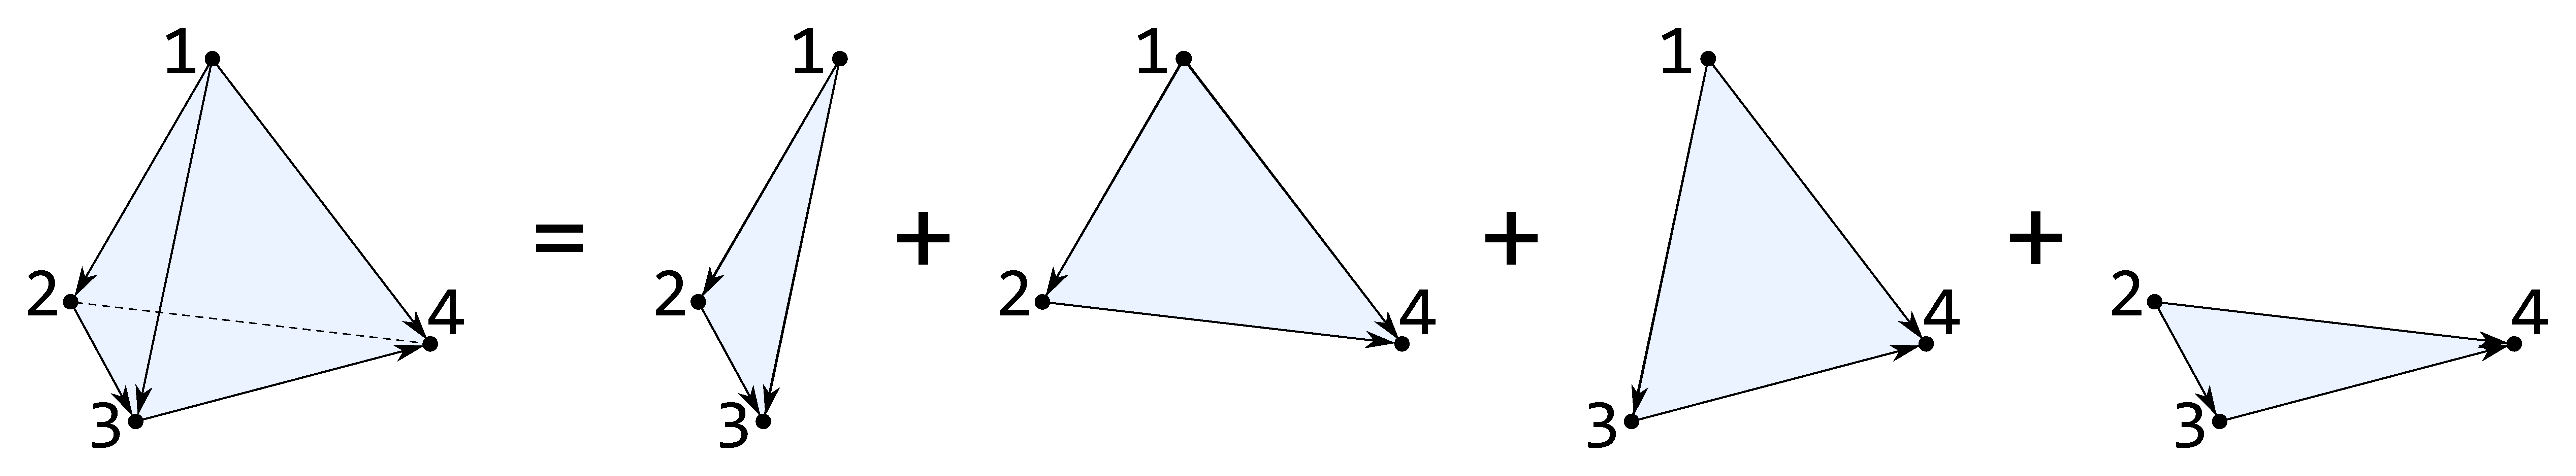
\includegraphics[scale=0.12]{fig/3-decomposition.pdf}}
\caption{3-decomposition:
    $1 \rightarrow 2 \rightarrow 3 \rightarrow 4 =
    1 \rightarrow 2 \rightarrow 3 + 1 \rightarrow 2 \rightarrow 4 +
    1 \rightarrow 3 \rightarrow 4 + 2 \rightarrow 3 \rightarrow 4$
    \label{fig-3-decomposition}}
\end{figure*}

\subsection{Reflexive graphs}\label{sub-reflexive}

A graph is \emph{reflexive} if every vertex of the graph is connected to itself,
i.e. has a self-loop. An example of a reflexive graph is the graph corresponding
to the partial order relation $\subseteq$ on graphs: indeed, $x \subseteq x$ holds
for all $x$. To represent reflexive graphs algebraically we can introduce the
following axiom:

\begin{itemize}
    \item Self-loop: $v = v \rightarrow v$, where $v\in \mathbb{V}$ is a vertex.
\end{itemize}

\noindent
The self-loop axiom corresponds to the additional \hs{Graph} law:

\begin{itemize}
    \item \hs{vertex x} = \hs{connect (}\hs{vertex x) (}\hs{vertex x)}.
\end{itemize}

One can implement the reflexive \hs{Graph} instance analogously to the
implementation of the \hs{Symmetric} data type presented in~\S\ref{sub-undirected},
by wrapping the \hs{Relation} into a \hs{newtype} and giving it a custom \hs{Eq}
instance based on the \hs{reflexiveClosure}.

We can define
\hs{class Graph@\,\,\blk{g}@ => ReflexiveGraph@\,\,\blk{g}@}
to increase the type safety of functions that rely on the self-loop axiom.

\subsection{Transitive graphs}\label{sub-transitive}

In many applications graphs satisfy the \emph{transitivity} property: if a vertex $x$ is
connected to $y$, and $y$ is connected to $z$, then the edge between $x$ and $z$ can be
added or removed without changing the semantics of the graph. A common example is
\emph{dependency graphs} or \emph{partial orders} --- the semantics of such graphs is
typically their \emph{transitive closure}.
To describe this class of graphs algebraically we add the following \emph{closure} axiom:

\begin{itemize}
    \item Closure: $y \neq \varepsilon \Rightarrow x \rightarrow y + y \rightarrow z +
    x \rightarrow z = x \rightarrow y + y \rightarrow z$.
\end{itemize}

By using the axiom one can rewrite a graph expression into its transitive closure or,
alternatively, into its \emph{transitive reduction}, hence all graphs that differ only in the
existence of some transitive edges are forced into the same equivalence class. Note that the
precondition $y \neq \varepsilon$ is necessary as otherwise $+$ and $\rightarrow$ can no
longer be distinguished, which is clearly undesirable:
\[
x\!\rightarrow\!z = x\!\rightarrow\!\varepsilon\!\rightarrow z = x\!\rightarrow\!\varepsilon
 + \varepsilon\!\rightarrow\!z + x\!\rightarrow\!z = x\!\rightarrow\!\varepsilon
 + \varepsilon\!\rightarrow\!z = x + z.
\]

It is interesting to note that $+$ and $\rightarrow$ have simple meanings for transitive
graphs: they correspond to the \emph{parallel} and \emph{sequential composition},
respectively. This allows to algebraically describe concurrent systems, which was
the original motivation behind the research on algebraic graphs~\cite{2014_algebra_mokhov}.

We can implement transitive graphs by wrapping
\hs{Relation} in a \hs{newtype Transitive} with a custom equality test that
compares the transitive closures of the underlying relations.
A subclass \hs{class Graph@\,\,\blk{g}@ => TransitiveGraph@\,\,\blk{g}@} can be
defined to distinguish algebraic graphs with the closure axiom from others.

\subsection{Preorders and equivalence relations}\label{sub-preorder}

By combining reflexive and transitive graphs, one can obtain \emph{preorders}.
For example, $(1 + 2 + 3) \rightarrow (2 + 3 + 4)$
is a preorder with vertices 2 and 3 forming a \emph{strongly-connected component}. By
finding all strongly-connected components in the graph (e.g. by utilising the
function \hs{scc} from the \textsf{containers} library) we can derive the
following \emph{graph condensation}:
$\{1\} \rightarrow \{2, 3\} \rightarrow \{4\}$. One way to interpret this preorder as a
dependency graph is that tasks 2 and 3 are executed as a step, simultaneously,
and that they both depend on task 1, and are prerequisite for task 4. Note that
having sets as the type of graph vertices is perfectly legal: the type of the
above graph condensation is \hs{(Graph g, Vertex g @\teq@ Set Int) => g}.

One can further combine preorders and undirected graphs, obtaining \emph{equivalence
relations}, which can be equipped with an efficient instance based on the
\emph{disjoint set} data structure~\cite{1984_set_union_tarjan}. One interesting
application of the resulting algebra is modelling connectivity in
circuits~\cite{2015_mokhov_algebra}.

\subsection{Hypergraphs}\label{sub-hypergraphs}

As described in~\S\ref{sub-relation}, the decomposition axiom collapses an algebraic
graph expression into a collection of vertices and pairs of vertices (i.e. graphs).
By replacing the decomposition axiom with \emph{3-decomposition}, we obtain
\emph{hypergraphs} comprising vertices, edges and \emph{3-edges} (triples of vertices):

\begin{itemize}
    \item 3-decomposition: $w \rightarrow x \rightarrow y \rightarrow z = \\
    w \rightarrow x \rightarrow y + w \rightarrow x \rightarrow z +
    w \rightarrow y \rightarrow z + x \rightarrow y \rightarrow z$.
\end{itemize}

Fig.~\ref{fig-3-decomposition} illustrates the axiom by decomposing a tetrahedron
into four 3-edges corresponding to its \emph{faces}. To better understand the
difference between the (2-)decomposition and 3-decomposition
axioms, let us substitute~$\varepsilon$ for $w$ in the 3-decomposition and simplify:
\[
x \rightarrow y \rightarrow z = x \rightarrow y + x \rightarrow z + y \rightarrow z
+ x \rightarrow y \rightarrow z.
\]
This is almost the 2-decomposition axiom, yet there is no way to get rid
of the term $x \rightarrow y \rightarrow z$ on the right-hand side: indeed, a triple is
unbreakable
in this algebra, and one can only extract the pairs (edges) that are embedded in it.
In fact, we can take this further and rewrite the above expression to also expose the
embedded vertices:
\[
x \rightarrow y \rightarrow z = x + y + z + x \rightarrow y + x \rightarrow z
+ y \rightarrow z + x \rightarrow y \rightarrow z.
\]
Note that with 2-decomposition we can achieve something similar via the absorption theorem:
\[
x \rightarrow y = x + y + x \rightarrow y.
\]
This can be taken further by defining 4-decomposition and so forth, creating a hierarchy
of algebraic structures corresponding to hypergraphs of different ranks.

Since every graph is also a hypergraph, we can define a superclass
\hs{class HyperGraph@\,\,\blk{g}@ => Graph@\,\,\blk{g}@}, moving all \hs{Graph} methods to the superclass, and
leaving only the decomposition axiom in \hs{Graph}, as the law that distinguishes it from
\hs{HyperGraph}.

% \subsection{Summary}

% In this section we have defined a family of graph instances and their classes that
% build on the algebraic core presented in~\S\ref{sec-algebra}. The additional axioms
% that characterise these classes
% can be mixed in various combinations. As an example, the algebra of undirected, reflexive
% and transitively closed graphs describes the laws of \emph{equivalence} relations and can be
% equipped with an
% efficient instance based on the \emph{disjoint set} data structure~\cite{1984_set_union_tarjan}.

% In the next section we present a library of basic graph transformation algorithms that
% can be reused by all graph instances discussed in this section.

%!TEX root = alga.tex
\begin{figure}
\begin{subfigure}[b]{0.27\linewidth}
\begin{minted}[fontsize=\small]{haskell}
class Graph g where
    type Vertex g
    empty   :: g
    vertex  :: Vertex g -> g
    overlay :: g -> g -> g
    connect :: g -> g -> g
\end{minted}
\caption{The core type class}
\end{subfigure}
\hfill
\hfill
\vrule
\hfill
\hfill
\begin{subfigure}[b]{0.68\linewidth}
\begin{minted}[fontsize=\small]{haskell}
vertices     :: Graph g => [Vertex g] -> g
edge         :: Graph g => Vertex g -> Vertex g -> g
edges        :: Graph g => [(Vertex g, Vertex g)] -> g
graph        :: Graph g => [Vertex g] -> [(Vertex g, Vertex g)] -> g
gen          :: (Graph g, Arbitrary (Vertex g)) => Gen g
isSubgraphOf :: (Graph g, Eq g) => g -> g -> Bool
\end{minted}
\caption{Derived graph construction primitives and the subgraph relation}
\end{subfigure}
~\\
~\\
\begin{subfigure}[b]{0.49\linewidth}
\begin{minted}[fontsize=\small]{haskell}
domain       @\,\,@::@\,\,@Relation a -> Set a
relation     @\,\,@::@\,\,@Relation a -> Set (a, a)
adjacencyMap @\,\,@::@\,\,@AdjacencyMap a -> Map a (Set a)
adjacencyList@\,\,@::@\,\,@AdjacencyMap a -> (a, [a])
edgeList     @\,\,@::@\,\,@AdjacencyMap a -> [(a, a)]
dfsForest    @\,\,@::@\,\,@AdjacencyMap a -> Forest a
topSort      @\,\,@::@\,\,@AdjacencyMap a -> Maybe [a]
\end{minted}
\caption{Deconstructing/consuming graphs}
\end{subfigure}
\hfill
\hfill
\vrule
\hfill
\hfill
\begin{subfigure}[b]{0.47\linewidth}
\begin{minted}[fontsize=\small]{haskell}
path   @\,\,@::@\,\,@Graph@\,\,\blk{g}@ => [Vertex g] -> g
circuit@\,\,@::@\,\,@Graph@\,\,\blk{g}@ => [Vertex g] -> g
clique @\,\,@::@\,\,@Graph@\,\,\blk{g}@ => [Vertex g] -> g
star   @\,\,@::@\,\,@Graph@\,\,\blk{g}@ => Vertex g -> [Vertex g] -> g
tree   @\,\,@::@\,\,@Graph@\,\,\blk{g}@ => Tree (Vertex g) -> g
forest @\,\,@::@\,\,@Graph@\,\,\blk{g}@ => Forest (Vertex g) -> g
fold   @\,\,@::@\,\,@(Graph@\,\,\blk{g}@,@\,@Vertex@\,\,\blk{g}\,\teq@@\,\blk{a}@)@\,\,@=>@\,\,@Expr@\,\,\blk{a}\,\,@->@\,\,\blk{g}@
\end{minted}
\caption{Standard families of graphs and graph folding}
\end{subfigure}
~\\
~\\
\begin{subfigure}[b]{\linewidth}
\begin{minted}[fontsize=\small]{haskell}
transpose     :: Transpose g -> g
toList        :: ToList a -> [a]
gmap          :: Graph g => (a -> Vertex g) -> GraphFunctor a -> g
mergeVertices :: Graph g => (Vertex g -> Bool) -> Vertex g -> GraphFunctor (Vertex g) -> g
bind          :: Graph g => GraphMonad a -> (a -> g) -> g
induce        :: Graph g => (Vertex g -> Bool) -> GraphMonad (Vertex g) -> g
removeVertex  :: (Graph g, Eq (Vertex g)) => Vertex g -> GraphMonad (Vertex g) -> g
splitVertex   :: (Graph g, Eq (Vertex g)) => Vertex g -> [Vertex g] -> GraphMonad (Vertex g) -> g
removeEdge    :: (Graph g, Eq (Vertex g)) => Vertex g -> Vertex g -> GraphMonad (Vertex g) -> g
box           :: (Graph g, Vertex g @\teq@ (u, v)) => GraphFunctor u -> GraphFunctor v -> g
deBruijn      :: (Graph g, Vertex g @\teq@ [a]) => Int -> [a] -> g
\end{minted}
\caption{Polymorphic graph transformations}
\end{subfigure}
\vspace{-3mm}
\caption{API of the graph transformation library\label{fig-api}}
\end{figure}

\newpage
\section{Graph transformation library}\label{sec-transformations}

In this section we demonstrate the flexibility of the algebraic graph core,
and develop a graph transformation library whose API is summarised in
Fig.~\ref{fig-api}. The parts of the API shown in Fig.~\ref{fig-api}(a-c)
were defined in~\S\ref{sec-algebra} and~\S\ref{sec-a-la-carte}.

\subsection{Standard families of graphs}\label{sub-families}

This subsection defines a few simple functions for constructing graphs from
standard graph families. An example is the family of \emph{clique} graphs that has
already been covered in \S\ref{sec-algebra}, where we defined the function
\hs{clique}. See Fig.~\ref{fig-api}(d) for the list of all functions we define.

A \emph{path} on a list of vertices can be constructed from the \hs{edges}
formed by the path neighbours:

\begin{minted}{haskell}
path :: Graph g => [Vertex g] -> g
path []  = empty
path [x] = vertex x
path xs  = edges $ @\std{zip}@ xs (@\std{tail}@ xs)
\end{minted}

\noindent
Note that the case with a single vertex on the path requires a special treatment.

If we connect the last vertex of a path to the first one, we get a \emph{circuit}
graph, or a \emph{cycle}. Let's express this in terms of the \hs{path} function:

\begin{minted}{haskell}
circuit :: Graph g => [Vertex g] -> g
circuit []     = empty
circuit (x:xs) = path $ [x] ++ xs ++ [x]
\end{minted}

A \emph{star} graph can be obtained by connecting a centre vertex to a given
list of \emph{leaves}:

\begin{minted}{haskell}
star :: Graph g => Vertex g -> [Vertex g] -> g
star x ys = connect (vertex x) (vertices ys)
\end{minted}

Finally, \emph{trees} and \emph{forests} can be constructed by the following
pair of mutually recursive functions:

\begin{minted}{haskell}
tree :: Graph g => Tree (Vertex g) -> g
tree (Node r f) = overlay (star r $ @\std{map}@ rootLabel f) (forest f)

forest :: Graph g => Forest (Vertex g) -> g
forest = @\std{foldr}@ overlay empty . @\std{map}@ tree
\end{minted}

\noindent
That is, a tree is represented by a star overlaid with the forest
of subtrees of the root's descendants. We remind the reader the
definitions of the data types \hs{Tree} and \hs{Forest} from the
\textsf{containers} library for completeness:

\begin{minted}{haskell}
data Tree a = Node { rootLabel :: a, subForest :: Forest a }

type Forest a = [Tree a]
\end{minted}

Below we experiment with these functions and their properties, and define
graphs \hs{pentagon} and \hs{p4} that will be used in subsection~\S\ref{sub-functor}
and in particular will feature in Fig.~\ref{fig-product}.

\begin{minted}[frame=single]{haskell}
@\ghci@ pentagon = circuit [1..5]
@\ghci@ p4 = path "abcd"

@\ghci@ :t pentagon
@\blk{pentagon}@ :: (Graph g, Num (Vertex g), Enum (Vertex g)) => g

@\ghci@ edgeList p4
[('a','b'),('b','c'),('c','d')]

@\ghci@ quickCheck $ \xs -> path xs `isSubgraphOf` (circuit xs :: Relation Int)
@\blk{+++ OK, passed 100 tests.}@

@\ghci@ adjacencyList $ forest $ dfsForest (1 + 2 * 3 + 4 * (5 + 6))
[(1,[@@]),(2,[3]),(3,[@@]),(4,[5,6]),(5,[@@]),(6,[@@])]

@\ghci@ quickCheck $ \xs -> path xs == (clique xs :: Transitive Int)
@\blk{+++ OK, passed 100 tests.}@
\end{minted}

The last property deserves a remark: the transitive closure of a path graph
is the clique on the same set of vertices, therefore they are considered equal
when interpreted by the \hs{Transitive} graph instance.

\subsection{Graph transpose}

In the rest of this section we present a toolbox for transforming polymorphic graph
expressions without turning them into a concrete data structure. The functions of the
presented toolbox are listed in Fig.~\ref{fig-api}(e).

One of the simplest transformations one can apply to a graph is to flip the
direction of all of its edges. It's usually straightforward to implement but
whatever data structure you use to represent graphs, you will spend at least
$O(1)$ time to modify it (say, by flipping the \hs{treatAsTransposed} flag);
much more often you will have to traverse the data structure and flip every edge,
resulting in $O(|V|+|E|)$ time complexity. However, by working with polymorphic
graphs, i.e. graphs of type \hs{forall g. Graph g => g}, and using Haskell's
zero-cost \hs{newtype} wrappers, we can implement transpose that takes zero time.

Consider the following \hs{Graph} instance:

\begin{minted}{haskell}
newtype Transpose g = T { transpose :: g } deriving (Arbitrary, Eq, Show)
\end{minted}
\vspace{1mm}
\begin{minted}{haskell}
instance Graph g => Graph (Transpose g) where
    type Vertex (Transpose g) = Vertex g
    empty       = T empty
    vertex      = T . vertex
    overlay x y = T $ overlay (transpose x) (transpose y)
    connect x y = T $ connect (transpose y) (transpose x) -- flip it!
\end{minted}

\noindent
That is, we wrap a graph in a \hs{newtype} flipping the order of \hs{connect} arguments.
Let's check if this works:

\begin{minted}[frame=single]{haskell}
@\ghci@ edgeList $ 1 * (2 + 3) * 4
[(1,2),(1,3),(1,4),(2,4),(3,4)]

@\ghci@ edgeList $ transpose $ 1 * (2 + 3) * 4
[(2,1),(3,1),(4,1),(4,2),(4,3)]
\end{minted}

This has zero runtime cost, because all we do is wrapping and unwrapping
the \hs{newtype}, which is guaranteed to be free or, more precisely, is handled
by the GHC at the compile time.

To make sure \hs{transpose} is only applied to polymorphic graphs, we do not export
the constructor \hs{T}, therefore the only way to call \hs{transpose} is to give it a
polymorphic argument and let the type inference interpret it as a value of type
\hs{Transpose}.

\subsection{Graph functor}\label{sub-functor}

We now implement a function \hs{gmap} that given a function \hs{a}~\hs{->}~\hs{b}
and a polymorphic graph whose vertices are of type \hs{a} will produce a
polymorphic graph with vertices of type \hs{b} by applying the function
to each vertex. This is almost a \hs{Functor} but it does not have the usual
type signature, because \hs{Graph} is not a higher-kinded type:

\vspace{2mm}
\begin{minted}{haskell}
newtype GraphFunctor a = GF { gfor :: forall g. Graph g => (a -> Vertex g) -> g }
\end{minted}
\vspace{1mm}
\begin{minted}{haskell}
instance Graph (GraphFunctor a) where
    type Vertex (GraphFunctor a) = a
    empty       = GF $ \_ -> empty
    vertex  x   = GF $ \f -> vertex (f x)
    overlay x y = GF $ \f -> overlay (gmap f x) (gmap f y)
    connect x y = GF $ \f -> connect (gmap f x) (gmap f y)
\end{minted}
\vspace{1mm}
\begin{minted}{haskell}
gmap :: Graph g => (a -> Vertex g) -> GraphFunctor a -> g
gmap = flip gfor
\end{minted}

Essentially, we are defining another newtype wrapper, which pushes the
given function all the way towards the vertices. This has no runtime cost,
just as before, although the actual evaluation of the given function at each
vertex will not be free, of course. Let's test this:

\begin{minted}[frame=single]{haskell}
@\ghci@ adjacencyList $ 1 * 2 * 3 + 4 * 5
[(1,[2,3]),(2,[3]),(3,[@@]),(4,[5]),(5,[@@])]

@\ghci@ adjacencyList $ gmap (+1) $ 1 * 2 * 3 + 4 * 5
[(2,[3,4]),(3,[4]),(4,[@@]),(5,[6]),(6,[@@])]
\end{minted}
\vspace{-1mm}
As you can see, we can increment the value of each vertex by mapping the function
\hs{(+1)} over the graph. The resulting expression is a polymorphic graph, as desired.
Again, we have done some useful work without turning the graph into a concrete data
structure. Note that \hs{gmap} satisfies the usual functor laws
\hs{gmap id = id} and \hs{gmap f@ . @}\hs{gmap g@ = @}\hs{gmap (f . g)}, because
it does not change the structure of the given graph expression and only pushes
the given function down to its leaves -- the vertices.

An alert reader might wonder: what happens if the function maps two different
vertices into the same one? They will be merged! Merging graph vertices is
a useful graph transformation, so let's define it in terms of \hs{gmap}:

\begin{minted}{haskell}
mergeVertices :: Graph g => (Vertex g -> Bool) -> Vertex g -> GraphFunctor (Vertex g) -> g
mergeVertices p v = gmap $ \u -> if p u then v else u
\end{minted}
\vspace{-1mm}
\begin{minted}[frame=single]{haskell}
@\ghci@ adjacencyList $ mergeVertices odd 3 $ 1 * 2 * 3 + 4 * 5
[(2,[3]),(3,[2,3]),(4,[3])]
\end{minted}
\vspace{-1mm}
The function takes a predicate on graph vertices and a target vertex and
maps all vertices satisfying the predicate into the target, thereby
merging them. In our example the \hs{odd} vertices $\{1, 3, 5\}$ are merged
into~3, in particular creating the self-loop $3 \rightarrow 3$. Note: it takes
linear time $O(|g|)$ for \hs{mergeVertices} to apply the predicate to each vertex
(where $|g|$ is the size of the graph expression $g$), which may be much more efficient
than merging vertices in a concrete data structure. For example, if the graph
is represented by an adjacency matrix, it will likely be necessary to rebuild
the resulting matrix from scratch, which takes $O(|V|^2)$ time. Since for
many graphs we have $|g| = O(|V|)$, our \hs{mergeVertices}
may be quadratically faster than the matrix-based one.

\begin{figure}
\centerline{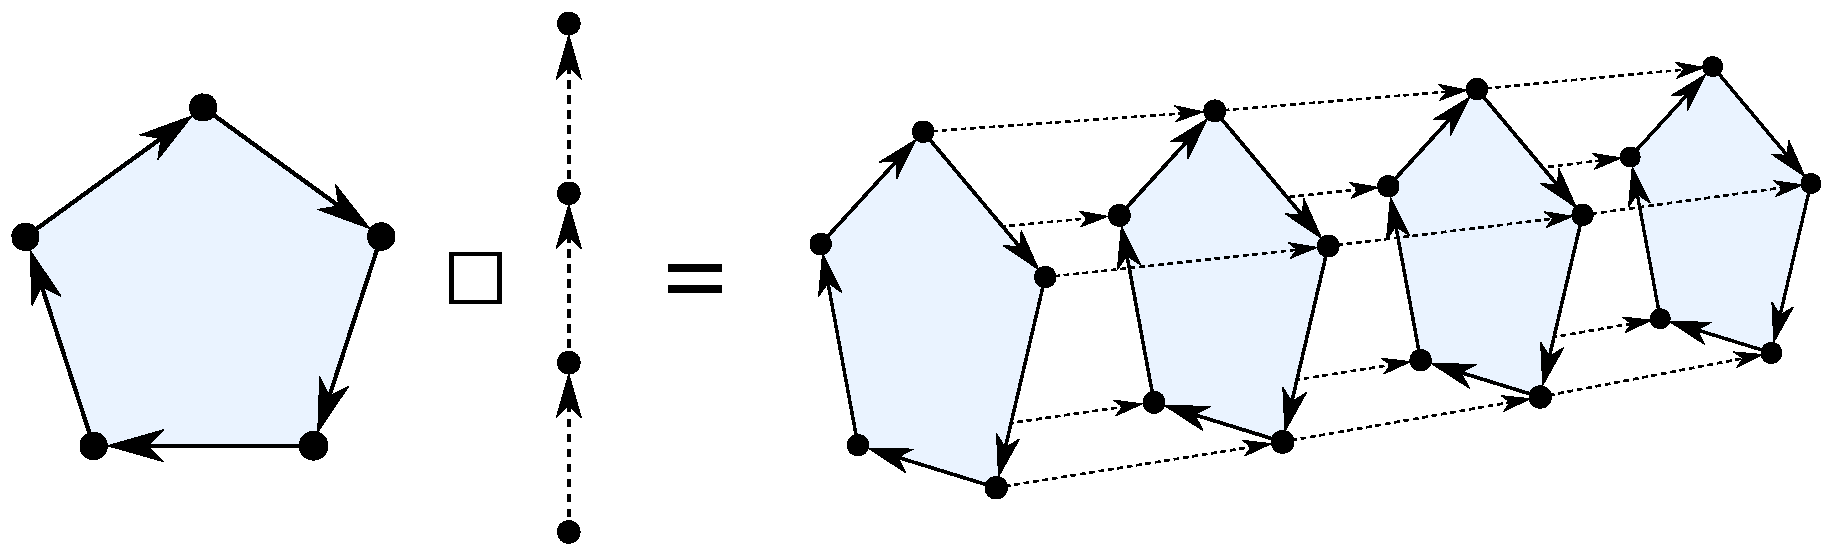
\includegraphics[scale=0.36]{fig/graph-product.pdf}}
\vspace{-4mm}
\caption{The Cartesian graph product of \hs{pentagon} and \hs{p4}, i.e. the graph
\hs{box@\,\,@}\hs{pentagon@\,\,@}\hs{p4}\label{fig-product}}
\vspace{-3mm}
\end{figure}

As another application of \hs{gmap}, we implement the \emph{Cartesian graph
product} operation \hs{box}, or $G~~\square~~H$, where the resulting vertex set is
$V_G \times V_H$ and vertex $(x, y)$ is connected to vertex $(x', y')$ if
either $x = x'$ and $(y, y') \in E_H$, or $y = y'$ and $(x,x')\in E_G$. An example of the Cartesian product of graphs \hs{pentagon}
and \hs{p4} is shown in Fig.~\ref{fig-product}.

\begin{minted}{haskell}
box :: (Graph g, Vertex g @\teq@ (u, v)) => GraphFunctor u -> GraphFunctor v -> g
box x y = @\std{foldr}@ overlay empty $ xs ++ ys
  where
    xs = @\std{map}@ (\b -> gmap (,b) x) . toList $ gmap id y
    ys = @\std{map}@ (\a -> gmap (a,) y) . toList $ gmap id x
\end{minted}

The Cartesian product $G~~\square~~H$ is assembled by creating $|V_H|$ copies
of graph $G$ and overlaying them with $|V_G|$ copies of graph $H$. We get
access to the list of graph vertices using \hs{toList} and turn vertices of
original graphs into pairs of vertices by \hs{gmap}. Note that we need to
\emph{reinterpret} the input of type \hs{GraphFunctor} as a polymorphic graph
by \hs{gmap@\,id@} before passing it to the \hs{toList} function, which expects
inputs of type \hs{ToList}. As you can see, we managed to implement quite
a sophisticated graph transformation function \hs{box} fully polymorphically.

The \hs{toList} function can be implemented by the following simple \hs{newtype}
wrapper:

\begin{minted}{haskell}
newtype ToList a = TL { toList :: [a] } deriving Show
\end{minted}
\vspace{1mm}
\begin{minted}{haskell}
instance Graph (ToList a) where -- note the lack of Eq a constraint
     type Vertex (ToList a) = a
     empty       = TL $ [@@]
     vertex  x   = TL $ [x]
     overlay x y = TL $ toList x ++ toList y
     connect x y = TL $ toList x ++ toList y
\end{minted}

\noindent
Note that we do not provide the \hs{Eq} instance for \hs{ToList}, because it
is impossible to make it law-abiding without requiring \hs{Eq} for vertices,
and we would like to avoid this in order to keep the \hs{box} type signature
fully parametric. As a consequence, \hs{toList (1 + 1)} produces the
list \hs{[1,1]}.

\subsection{Graph monad}\label{sub-monad}

What do the operations of removing a vertex and splitting a vertex have in common?
They both can be implemented by replacing each vertex of a graph with a (possibly empty)
subgraph and flattening the result. You may recognise this as monad's
\hs{bind} operation. We are going to implement \hs{bind}
by wrapping it into yet another \hs{newtype}:

\begin{minted}{haskell}
newtype GraphMonad a = GM { bind :: forall g. Graph g => (a -> g) -> g }
\end{minted}
\vspace{1mm}
\begin{minted}{haskell}
instance Graph (GraphMonad a) where
    type Vertex (GraphMonad a) = a
    empty       = GM $ \_ -> empty
    vertex  x   = GM $ \f -> f x -- here is the difference from gmap
    overlay x y = GM $ \f -> overlay (bind x f) (bind y f)
    connect x y = GM $ \f -> connect (bind x f) (bind y f)
\end{minted}

As you can see, the implementation is almost identical to \hs{gmap}: instead of
wrapping the value \hs{f@\,\,@x} into a \hs{vertex}, we should just leave it as is.
Let's see how we can make use of this new type in our toolbox.

Firstly, we are going to implement a \hs{@\std{filter}@}-like function \hs{induce}
that, given a vertex predicate and a graph, will compute the \emph{induced subgraph}
on the set of vertices that satisfy the predicate by turning all other
vertices into empty subgraphs and flattening the result.

\begin{minted}{haskell}
induce :: Graph g => (Vertex g -> Bool) -> GraphMonad (Vertex g) -> g
induce p g = bind g $ \v -> if p v then vertex v else empty
\end{minted}
\vspace{1mm}
\begin{minted}[frame=single]{haskell}
@\ghci@ edgeList $ clique [0..4]
[(0,1),(0,2),(0,3),(0,4),(1,2),(1,3),(1,4),(2,3),(2,4),(3,4)]

@\ghci@ edgeList $ induce (<3) $ clique [0..4]
[(0,1),(0,2),(1,2)]
\end{minted}

\noindent
As you can see, by inducing a clique on a subset of the vertices
that we like \hs{(<3)}, we get a smaller clique, as expected.
The cost of \hs{induce} for a given expression $g$ is $O(|g|)$.

We can now -- at last -- implement the \hs{removeVertex} function, as
was promised in the motivation section~\S\ref{sec-motivation}.

\begin{minted}{haskell}
removeVertex :: (Graph g, Eq (Vertex g)) => Vertex g -> GraphMonad (Vertex g) -> g
removeVertex v = induce (/= v)
\end{minted}
\vspace{1mm}
\begin{minted}[frame=single]{haskell}
@\ghci@ adjacencyList $ removeVertex 2 $ 1 * 2 + 3 * 1
[(1,[@@]),(3,[1])]
\end{minted}

\noindent
Note that the above example matches the one in Fig.~\ref{fig-example}.

The polymorphic implementation of \hs{removeVertex} presented above takes
$O(|g|)$ to remove a vertex from a graph expression $g$, which is
slower than some concrete data structures.

We can also use the \hs{bind} function to split a vertex into a list of given vertices:

\begin{minted}{haskell}
splitVertex :: (Graph@\,\,g@,@\,@Eq@\,@(Vertex@\,\,g@)) => Vertex@\,\,g@ -> [Vertex@\,\,g@] -> GraphMonad@\,@(Vertex@\,\,g@) -> g
splitVertex v vs g = bind g $ \u -> if u == v then vertices vs else vertex u
\end{minted}
\vspace{1mm}
\begin{minted}[frame=single]{haskell}
@\ghci@ adjacencyList $ splitVertex 1 [0, 1] $ 1 * (2 + 3)
[(0,[2,3]),(1,[2,3]),(2,[@@]),(3,[@@])]
\end{minted}

\noindent
Here vertex 1 is split into a pair of vertices $\{0, 1\}$ that have the same connectivity.

\subsection{Beyond homomorphisms}\label{sub-beyond}

Most of the \hs{newtype} wrappers defined in this section are \emph{homomorphisms},
that is, they preserve the structure of the original graph expression. The two
exceptions are: \hs{Transpose}, which is an \emph{antihomomorphism}, and
\hs{ToList} which collapses the structure of the original expression into a list.

Below we derive an implementation for \hs{removeEdge}, which is another
example of a useful function that is not a homomorphism. Removing an edge sounds
easy, but the result is the most complicated \hs{newtype} in this paper.

\begin{minted}{haskell}
newtype RemoveEdge a = RE { re :: forall g. (Vertex g @\teq@ a, Graph g) => a -> a -> g }
\end{minted}
\vspace{1mm}
\begin{minted}{haskell}
instance Eq a => Graph (RemoveEdge a) where
    type Vertex (RemoveEdge a) = a
    empty       = RE $ \_ _ -> empty
    vertex  x   = RE $ \_ _ -> vertex x
    overlay x y = RE $ \u v -> overlay (re x u v) (re y u v)
    connect x y = RE $ \u v -> connect (removeVertex u $ re x u u) (re y u v) `overlay`
                               connect (re x u v) (removeVertex v $ re y v v)
\end{minted}
\vspace{1mm}
\begin{minted}{haskell}
removeEdge :: (Eq@\,@(Vertex g),@\,@Graph g) => Vertex g -> Vertex g -> RemoveEdge@\,@(Vertex g) -> g
removeEdge u v g = re g u v
\end{minted}

\noindent
Here is how it works. Removing an edge from the \hs{empty} graph or a \hs{vertex} is easy:
nothing needs to be done, because there are no edges. To remove an edge from an
\hs{overlay}, we simply recurse to both subexpressions -- the overlay does not create
any edges.

\begin{minted}[frame=single]{haskell}
@\ghci@ edgeList $ path "Hello"
[('H','e'),('e','l'),('l','l'),('l','o')]

@\ghci@ edgeList $ removeEdge 'H' 'e' $ path "Hello"
[('e','l'),('l','l'),('l','o')]

@\ghci@ edgeList $ removeEdge 'l' 'l' $ path "Hello"
[('H','e'),('e','l'),('l','o')]
\end{minted}

\subsection{Benchmarks}\label{sub-benchmarks}


%!TEX root = alga.tex
\section{Related work}\label{sec-related}

Historically, first approaches to graph representation in functional programming
used edge lists, adjacency lists, as well as mutually recursive data structures
representing cyclic graphs by the so-called `tying the knot' approach. The former
were generally slower
than their imperative counterparts, while the latter were very difficult to
work with. An asymptotically optimal implementation of the depth-first search
algorithm developed by~\citet{1995_king_graphs} used arrays to represent graphs
and \emph{state-transformer monads}~\cite{1994_launchbury_st} to mimic imperative array
updates in pure functional programming. The developed algorithms are still in
use today and are available from the \textsf{containers} library shipped with the GHC.
As demonstrated in the motivation section~\S\ref{sec-motivation}, the API of
the library is difficult to use and contains partial functions.

A fundamentally different approach by~\citet{2001_erwig_inductive} is based
on \emph{inductive graphs}, whereby a graph can be decomposed into a \emph{context}
(a node with its neighbourhood) and the rest of the graph. This inductive
definition makes it possible to share common subgraphs and provides a way to
implement graph algorithms in a more functional style compared to the previous
approaches based on array representations. Inductive graphs are implemented in
the \textsf{fgl} library that contains implementations of many standard graph
algorithms, from depth-first search to maximum flow on weighted graphs. Compared
to algebraic graphs proposed in this paper, the \textsf{fgl} library has a larger
core of graph construction primitives (10 vs 4), some of which are partial, as
has been shown in the motivational example in \S\ref{sec-motivation}.

Several other authors investigated ways to define graphs compositionally,
e.g.~\citet{1995_gibbons_algebra} proposed an algebraic framework for modelling
acyclic graphs comprising 6 core graph construction primitives, but the approach
was not general enough to handle other practically useful classes of graphs.

From a very different angle, simple algebraic structures, such as \emph{semirings},
have been successfully applied to solving various path problems on graphs using
functional programming, e.g. see~\citet{2013_semirings_dolan}. These approaches
typically use matrix-based data structures for manipulating connectivity and distance
information with the goal of solving optimisation problems on graphs, and are not
suitable as an abstract interface for graph representation.

This paper builds on the work by~\citet{2014_algebra_mokhov}, where
the \emph{algebra of parameterised graphs}, a mathematical
structure very similar to a semiring, was proposed as a complete and sound formalism
for graph representation in the context of digital circuit design. The authors did
not investigate applications of the algebra in functional programming but proved
many important results that are essential for this paper.
\citet{2014_alekseyev_phd} derived a formalisation of the algebra of parameterised
graphs in the Agda programming language, using an encoding similar to
the core type class that we define.

% \begin{itemize}
%     \item Structured Graphs by Oliveira & Cook. \url{https://www.cs.utexas.edu/~wcook/Drafts/2012/graphs.pdf}
%     \item "Algebras for graphs have been studied in the context of graph rewriting, see Bauderon and Courcelle (1986), for example."
% \end{itemize}

%!TEX root = alga.tex
\section{Discussion, limitations and future research}\label{sec-discussion}

The paper presented \emph{algebraic graphs} --- a new approach to representing and
working with graphs in functional programming languages.
Compared to the state-of-the-art, algebraic graphs are easier to use,
more compositional, and have a smaller core of only four graph
construction primitives characterised by an elegant algebra of graphs.

We demonstrated the flexibility of algebraic graphs by numerous examples and
developed a library for polymorphic graph construction and transformation.

The presented approach has a few limitations:

\begin{itemize}
    \item There are no known efficient implementations of fundamental graph
    algorithms, such as depth-first search, that work directly on the algebraic
    core. Therefore, we need to translate core expressions to conventional
    graph representations, such as adjacency lists, and utilise existing graph
    libraries, which may be suboptimal for certain algorithmic problems.

    \item Many of the presented \hs{Graph} instances incur a logarithmic overhead
    during graph construction and therefore do not scale well. The performance
    figures reported in~\S\ref{sub-library-summary} are not acceptable for
    high-performance applications. A promising direction to overcoming this limitation
    is to employ the \emph{discrimination} Haskell library that provides linear-time
    sorting and grouping algorithms~\cite{2012_henglein_discriminations}.

    \item This paper has not addressed labelled graphs. In particular, there is
    no known algebraic characterisation of
    graphs with arbitrary vertex and edge labels. However,~\citet{2014_algebra_mokhov}
    give an algebraic characterisation for graphs labelled with Boolean functions.
    % \item The graph transformation library does not provide the functionality
    % for overriding the default implementation of functions that can be implemented
    % more efficiently by a specific data structure. An example of a function that
    % would particular benefit from overriding is \hs{removeEdge}, as defined
    % in~\S\ref{sub-beyond}.
\end{itemize}

Despite these limitations, algebraic graphs have been successfully used
in the design of asynchronous circuits~\cite{2015_beaumont_concepts} and
processor microcontrollers~\cite{2014_algebra_mokhov}.

Our future research will focus on addressing the above limitations, and on
exploration of the following topics:

\begin{itemize}
    \item By using the algebraic approach to graph representation one can
    formulate graph algorithms in the form of solving systems of algebraic
    equations with unknowns.
    This may potentially open way to the discovery of novel graph algorithms.
    \item Algebraic graph expressions can be minimised via the
    \emph{modular decomposition} of graphs~\cite{2005_mcconnell_modular}, thereby
    reducing their memory footprint, as well as speeding up their processing.
    Exploiting the compactness of algebraic graphs in algorithms is a
    promising research direction.
\end{itemize}


%% Acknowledgments
\begin{acks}                            %% acks environment is optional
                                        %% contents suppressed with 'anonymous'
  %% Commands \grantsponsor{<sponsorID>}{<name>}{<url>} and
  %% \grantnum[<url>]{<sponsorID>}{<number>} should be used to
  %% acknowledge financial support and will be used by metadata
  %% extraction tools.
  This material is based upon work supported by the
  \grantsponsor{GS100000001}{National Science
    Foundation}{http://dx.doi.org/10.13039/100000001} under Grant
  No.~\grantnum{GS100000001}{nnnnnnn} and Grant
  No.~\grantnum{GS100000001}{mmmmmmm}.  Any opinions, findings, and
  conclusions or recommendations expressed in this material are those
  of the author and do not necessarily reflect the views of the
  National Science Foundation.
\end{acks}

\bibliography{publications}

% \appendix
% \section{Appendix}

% Text of appendix \ldots

\end{document}
